\section{Experiment}
\label{sec:experiment}

\subsection{Dataset and Features}
\label{sec:dataset}

% experiment protocol: Nested cross-validation with Monte-Carlo cross-validation for the inner loop
We experiment methods developed in Section~\ref{sec:trajrec} on trajectories extracted from Flickr photos~\cite{thomee2016yfcc100m}.
The statistics of datasets are shown in Table~\ref{tab:data} and 
the histograms of the number of ground truths for queries are shown in Figure~\ref{fig:hist}.

% dataset stats
\begin{table}[t]
\caption{Statistics of trajectory dataset}
\label{tab:data}
\centering
\setlength{\tabcolsep}{4pt} % tweak the space between columns
\begin{tabular}{l*{5}{r}} \hline
\textbf{Dataset} & \textbf{\#Photos} & \textbf{\#Visits} & \textbf{\#Traj.} & \textbf{\#Users} & \textbf{\#Queries} \\ \hline
Edinburgh & 82,060 & 33,944 & 5,028 & 1,454 & 147 \\
Glasgow & 29,019 & 11,434 & 2,227 & 601 & 64 \\
Melbourne & 94,142 & 23,995 & 5,106 & 1,000 & 280 \\
Osaka & 392,420 & 7,747 & 1,115 & 450 & 47 \\
Toronto & 157,505 & 39,419 & 6,057 & 1,395 & 99 \\
\hline
\end{tabular}
\end{table}


% histogram of #ground truth
\begin{figure*}[t]
	\centering
	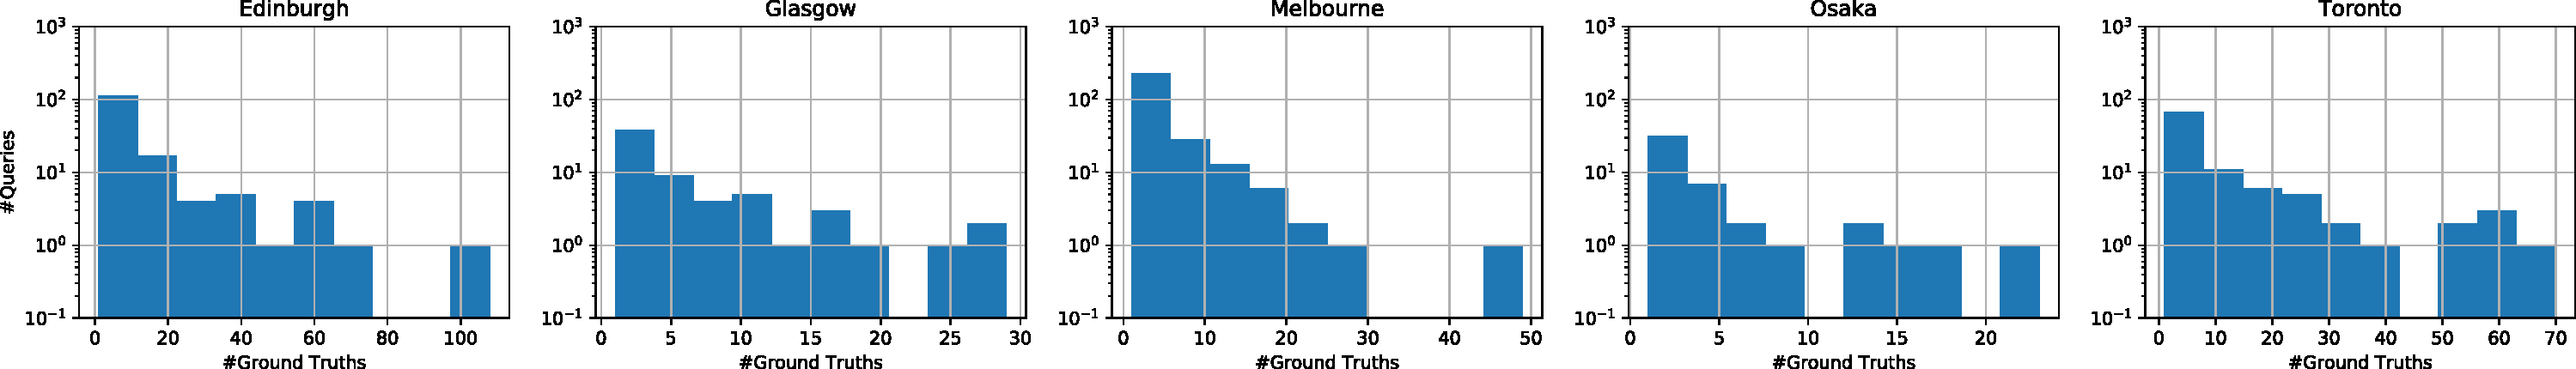
\includegraphics[width=\textwidth]{hist.pdf}
	\caption{Histogram of the number of ground truth}
	\label{fig:hist}
\end{figure*}


% leave-one-out evaluation (with query aggregation)
As described in Section~\ref{sec:queryagg}, 
we first group trajectories according to queries that they conform to,
then evaluate the performance of each algorithm using leave-one-out cross validation,
where we hold each query and its associated trajectories for test and all other trajectories for training.
% model selection (Monte Carlo CV) (with query aggregation): 90/10 random split for 5 times
Furthermore, 
the hyper-parameter (regularisation constant $C$) is tuned using the Monte Carlo cross validation~\cite{burman1989comparative} on training set.

% evaluation metric: kendall's Tau (mention F1, pF1)
To evaluate the performance of each algorithm variant, 
we compute the Kendall's $\tau$ (version $b$)~\cite{kendall1945,agresti2010analysis} to measure the quality of recommendation.
In particular,
we define the rank of POIs $\mathcal{P}$ given trajectory $\mathbf{y} = (y_1,\dots,y_K)$ as
\begin{align*} 
r_\mathbf{y} &= (r_1,\dots,r_j,\dots,r_{|\mathcal{P}|}), \\
r_j &= \sum_{k=1}^K (| \mathcal{P} | - k + 1)  \llb p_j = y_k \rrb, ~ j = 1, \dots, | \mathcal{P} |.
\end{align*}
Unlike the F$_1$ sore on points~\cite{ijcai15} or the F$_1$ score on pairs~\cite{cikm16paper}, 
which only cares about either the set of correctly recommended POIs or the set of correctly predicted POI pairs,
this metric taking both factors into account.

In addition, we take the maximum of all pairs,
i.e.,
\begin{equation*}
\tau_b^{(i)} = 
\max_{(\mathbf{y}, \hat{\mathbf{y}}) \in \{\mathbf{y}^{(ij)}\}_{j=1}^{N_i} \times \{\hat{\mathbf{y}}^{(ij)}\}_{j=1}^k} 
\tau_b(r_\mathbf{y}, r_{\hat{\mathbf{y}}}),
\end{equation*}
where $\{\mathbf{y}^{(ij)}\}_{j=1}^{N_i}$ are the ground truths for query $\mathbf{x}^{(i)}$ and
$\{\hat{\mathbf{y}}^{(ij)}\}_{j=1}^k$ are the top-$k$ recommendations.



\subsection{Experimental Results}
\label{sec:result}

% algorithms
We evaluate the recommender based on standard structured prediction (\textsc{SP}), 
the structured recommender with query aggregation (\textsc{SR}) and 
their variants with sub-tour elimination when training these recommender systems,
i.e., \textsc{SPpath} and \textsc{SRpath}, respectively.
In addition, we looked at three baselines including \textsc{Random} which simply recommend random POIs according to query.

% experimental results
The results of experiment on five trajectory datasets are shown in Table~\ref{tab:tau}.

\begin{table*}[t]
\caption{Kendall's $\tau$}
\label{tab:tau}
\centering
\begin{tabular}{l|ccccc} \hline
 & Osaka & Glasgow & Edinburgh & Toronto & Melbourne \\ \hline
\textsc{Random} & $0.403\pm0.025$ & $0.410\pm0.032$ & $0.374\pm0.021$ & $0.416\pm0.026$ & $0.324\pm0.012$ \\
\textsc{Popularity} & $0.567\pm0.034$ & $0.646\pm0.035$ & $\mathbf{0.668\pm0.020}$ & $0.625\pm0.023$ & $0.491\pm0.014$ \\
\textsc{PoiRank} & $0.646\pm0.040$ & $0.736\pm0.030$ & $0.663\pm0.020$ & $0.721\pm0.024$ & $0.503\pm0.013$ \\
\textsc{SP} & $0.796\pm0.037$ & $0.865\pm0.027$ & $0.664\pm0.020$ & $\mathbf{0.803\pm0.022}$ & $\mathbf{0.527\pm0.018}$ \\
\textsc{SPpath} & $0.794\pm0.035$ & $0.740\pm0.034$ & $-$ & $-$ & $-$ \\
\textsc{SR} & $\mathbf{0.814\pm0.034}$ & $\mathit{0.870\pm0.025}$ & $\mathit{0.667\pm0.022}$ & $\mathit{0.792\pm0.022}$ & $\mathit{0.508\pm0.018}$ \\
\textsc{SRpath} & $\mathit{0.805\pm0.036}$ & $\mathbf{0.877\pm0.025}$ & $-$ & $-$ & $-$ \\
\hline
\end{tabular}
\end{table*}

We can see from the empirical results that all variants of structured prediction recommender achieve very good performance.
In particular, recommendations based on standard SSVM (\textsc{SP}) are comparable to those based on structured recommender (\textsc{SR}), 
which means query aggregation does not hurt recommendation but also provide any significant benefit.

Another observation is that training a structured recommender with sub-tour elimination does not help the quality of recommendations,
besides, sub-tour elimination make the training computationally expensive, which makes the evaluation on large datasets 
(e.g., Edinburgh, Melbourne and Toronto) impractical.

It is interesting to see that both the \textsc{Popularity} and \textsc{PoiRank} perform very well on both Edinburgh and Melbourne,
in particular, \textsc{Popularity} is the best performer on Edinburgh, which indicates that most tourists travelling following the degree 
of popular of each place.
